% \documentclass[fleqn]{jsarticle}

% \usepackage{graphicx}
% \usepackage{amsmath,amssymb}
% \usepackage{amsmath}
% \usepackage{fancyhdr}

\documentclass[dvipdfmx]{jsarticle}
\usepackage[dvipdfmx]{graphicx}
\usepackage{color}
\usepackage{amsmath}
\usepackage{amsfonts}
\usepackage{circuitikz}
\usepackage{cases}
\usepackage{otf}
\usepackage{ascmac,multicol,pifont,url}
\usepackage{booktabs}
\usepackage{bm}
\usepackage{listings,jlisting}
\usepackage{fancyhdr}



\pagestyle{fancy}
\fancyhead[RE,RO]{先端データ解析論 レポート}

\usepackage{xcolor}
\usepackage[justification=centering]{caption}
\usepackage{listings}
\renewcommand{\lstlistingname}{リスト}
\lstset{language=Python,%
        % basicstyle=\footnotesize,%
        basicstyle=\tiny,%
        commentstyle=\textit,%
        classoffset=1,%
        keywordstyle=\bfseries,%
      	frame=tRBl,framesep=5pt,%
      	showstringspaces=false,%
        linewidth=38em,
      	}%



% \DeclareMathOperator*{\argmin}{argmin}
\newcommand{\bmu}{{\bm{\mu}}}
\newcommand{\bmut}{\bm{\mu}^\top}
\newcommand{\tbmu}{\tilde{\bm{\mu}}}
\newcommand{\hbmu}{\hat{\bm{\mu}}}
\newcommand{\hbmut}{\hat{\bm{\mu}}^\top}
\newcommand{\tbmut}{\tilde{\bm{\mu}}^\top}
\newcommand{\sig}{\tilde{\bm{\Sigma}}}
\newcommand{\siginv}{\tilde{\bm{\Sigma}}^{-1}}
\newcommand{\bphi}{\bm{\phi}(\bm{x})}
\newcommand{\bphit}{\bm{\phi}(\bm{x})^\top}

\newcommand{\ex}{\mathbb{E}}
\newcommand{\bmx}{\bm{x}}
\newcommand{\bmxd}{\bm{x}{'}}
\newcommand{\ptrain}{p_{\text{train}}}
\newcommand{\hoge}{\mathbb{E}_{\bmxd \sim p_{\text{test}}, \bmx \sim q_\pi}}
\newcommand{\fuga}{\mathbb{E}_{\bmxd, \tilde{\bmx}' \sim p_{\text{test}}}}
\newcommand{\piyo}{\mathbb{E}_{\bmx, \tilde{\bmx} \sim q_\pi}}


\newcommand{\argmax}{\mathop{\rm argmax}\limits}
\newcommand{\argmin}{\mathop{\rm argmin}\limits}

\title{先端データ解析論 第9回レポート}
\author{電子情報学専攻 48-176403 石毛真修}


\begin{document}
\maketitle


\section*{大問1.}
ガウスカーネルモデルを用いた,ラプラス正則化最小二乗確率的分類を実装する.
まず,学習するデータを生成する関数と,学習結果を等高線グラフとして描画する関数を定義する.
\begin{center}
\begin{tabular}{c}
  \begin{lstlisting}[]
    import numpy as np
    from numpy.random import seed, randn


    def create_data(n):
        points = np.linspace(0, np.pi, n // 2)
        u = - 10 * np.concatenate([np.cos(points) + 0.5, np.cos(points) - 0.5]).reshape(n, 1) + randn(n, 1)
        v = 10 * np.concatenate([np.sin(points), - np.sin(points)]).reshape(n, 1) + randn(n, 1)
        X = np.array([u, v]).reshape(2, n).transpose((1, 0))
        y = np.zeros((n, 1))
        y[0] = - 1
        y[-1] = 1
        return X, y


    def draw_contour(axis_range=(-20, 20), granularity=100, z_func=lambda x, y: x + y):
        # You have to plt.show() after this function
        axis = np.linspace(*axis_range, granularity)
        X, Y = np.meshgrid(axis, axis)
        Z = z_func(X, Y)
        plt.contourf(X, Y, Z)

  \end{lstlisting}
\end{tabular}{c}
\end{center}

カーネル行列やカーネル関数を生成するのに必要な関数を定義する.
\begin{center}
  \begin{tabular}{c}
  \begin{lstlisting}[]
    def kernel_matrix(X, rows=None, h=1.):
        """
        X: [(x0[0], x0[1]), (x1[0], x1[1]), ...]
        """
        if rows is None:
            return np.exp(- dist_matrix(X) / (2 * h**2))
        else:
            return np.exp(- dist_matrix(X)[:rows] / (2 * h**2))


    def kern(x, train_X, h=1.):
        """
        x: [(x0[0], x0[1]), (x1[0], x1[1])]
        X: [(x0[0], x0[1]), (x1[0], x1[1]), ...]
        """
        x_sq = tile_square(x, train_X.shape[0])
        X_sq = tile_square(train_X, x.shape[0]).transpose((1, 0))
        dist = x_sq + X_sq - 2 * x @ train_X.T
        return np.exp(- dist / (2 * h**2))


    def tile_square(X, cols):
        """
        Align X^2 colum-wise
        X: [(x0[0], x0[1]), (x1[0], x1[1]), ...]
        """
        sq = np.square(X[:, 0]) + np.square(X[:, 1])
        sq = sq.reshape([X.shape[0], 1])
        return np.tile(sq, cols)


    def dist_matrix(X):
        """
        X: [(x0[0], x0[1]), (x1[0], x1[1]), ...]
        Returns: [[(x0 - x0)^2, (x0 - x1)^2, ...], ...]
        """
        sq = tile_square(X, X.shape[0])
        return sq + sq.T - 2 * X @ X.T
  \end{lstlisting}
\end{tabular}{c}
\end{center}

ラプラス行列を生成する関数を定義する.
\begin{center}
  \begin{tabular}{c}
  \begin{lstlisting}[]
    def weight_matrix(X, k=10):
        """
        X: [(x0[0], x0[1]), (x1[0], x1[1]), ...]
        k: k nearest neighbor
        """
        n = X.shape[0]
        W = np.zeros((n, n))
        dist = dist_matrix(X)
        for i in range(n):
            for j in range(i + 1, n):
                if is_mutually_k_nearest(dist, i, j, k):
                    W[i, j] = 1.
                    W[j, i] = 1.
        return W


    def is_mutually_k_nearest(dist_matrix, i: int, j: int, k: int):
        """
        dist_matrix: [[d(x0, x0), (x0, x1), ...], [d(x1, x0), (x1, x1), ...], ...]
        """
        # Is j k-nearest-neighbour of i ?
        dist_from_i = dist_matrix[i]
        k_nearest_idxes = np.argsort(dist_from_i)[:k + 1]
        if j not in k_nearest_idxes:
            return False
        # Is i k-nearest-neighbour of j ?
        dist_from_j = dist_matrix[j]
        k_nearest_idxes = np.argsort(dist_from_j)[:k + 1]
        if i not in k_nearest_idxes:
            return False
        return True


    def laplacian_matrix(X, k=10):
        W = weight_matrix(X, k)
        D = np.diag(np.sum(W, axis=1))
        return D - W
  \end{lstlisting}
\end{tabular}{c}
\end{center}

パラーメタ$\theta$を推定し,分類器を生成する.
\begin{center}
  \begin{tabular}{c}
  \begin{lstlisting}[]
    def estimate_theta(labeled_X, labels, unlabeled_X, k=2, lamb=1., nu=1.):
        """
        X: [(x0[0], x0[1]), (x1[0], x1[1]), ...]
        """
        X = np.concatenate((labeled_X, unlabeled_X))
        K = kernel_matrix(X)
        K_l = kernel_matrix(X, labeled_X.shape[0])
        L = laplacian_matrix(X, k)

        Q = K_l.T @ K_l + lamb * np.eye(X.shape[0]) + 2 * nu * K.T @ L @ K
        return np.linalg.inv(Q) @ K_l.T @ labels


    def generate_classifier(theta, train_X):
        def classifier(X0, X1):
            """
            X0: [[p0, p1, ...], [...], ...]
            X1: [[q0, q1, ...], [...], ...]
            """
            X = np.array([X0, X1]).transpose((1, 2, 0)).reshape(-1, 2)
            kernels = kern(X, train_X)
            signs = np.array(np.sign(kernels @ theta))
            reshaped = np.array(np.split(signs.reshape(-1), X0.shape[0]))
            return reshaped
        return classifier
  \end{lstlisting}
\end{tabular}{c}
\end{center}

以上をまとめて実行する.
\begin{center}
  \begin{tabular}{c}
    \begin{lstlisting}[]
      def main():
          seed(42)
          X, y = create_data(200)
          labeled_X = X[(y != 0).reshape(-1)]
          unlabeled_X = X[(y == 0).reshape(-1)]
          labels = y[(y != 0).reshape(-1)]
          t = estimate_theta(labeled_X, labels, unlabeled_X, 4)
          classifier = generate_classifier(t, X)

          draw_contour(granularity=500, z_func=classifier)
          plt.plot(X[(y == 1).reshape(-1), 0], [X[(y == 1).reshape(-1), 1]], 'bo')
          plt.plot(X[(y == -1).reshape(-1), 0], [X[(y == -1).reshape(-1), 1]], 'rx')
          plt.plot(X[(y == 0).reshape(-1), 0], X[(y == 0).reshape(-1), 1], '.')
          plt.show()

      main()
    \end{lstlisting}
  \end{tabular}{c}
\end{center}

実行すると次のような結果を得る.
\begin{figure}[h]
  \begin{center}
    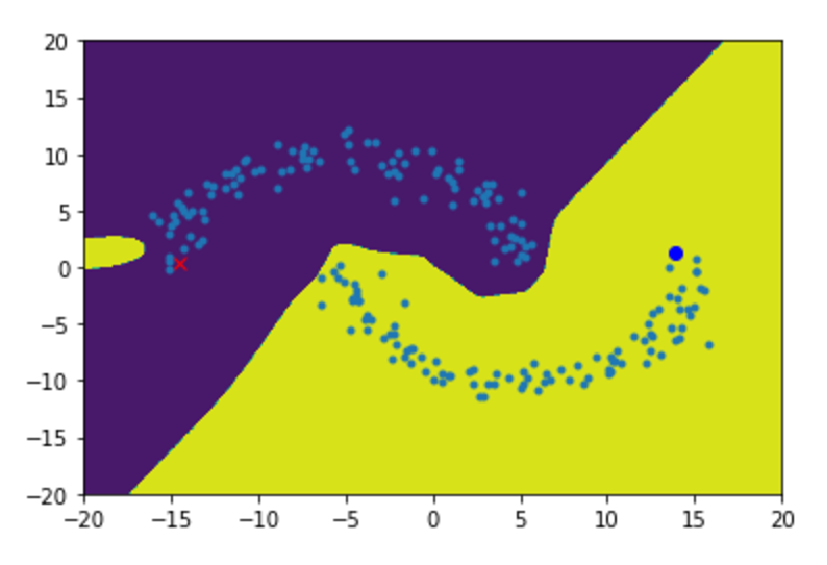
\includegraphics[width=0.6\textwidth]{figs/laplacian_normalization_result.eps}
  \end{center}
  \caption{ラプラス正則化最小自乗分類による半教師あり学習の結果}
\end{figure}
若干分類に失敗している部分が見受けられる.

\newpage

\section*{大問2}

エネルギー距離の2乗の式
$$
D_E^2 (p_{\text{test}}, q_\pi) = 2 \underbrace{\hoge||\bmxd - \bmx||}_{(1)}
- \underbrace{\fuga||\bmxd - \tilde{\bmx}'||}_{(2)}
- \underbrace{\piyo||\bmx - \tilde{\bmx}||}_{(3)}
$$
について,各項を変形する.%以下では表記を簡単にするために,例えば$\ptrain(\bmx | y = 1)$を$\ptrain(y = 1)$のように略記することとする.

\begin{eqnarray*}
 \hoge||\bmxd - \bmx|
 &=& \iint p_\text{test}(\bmx') q_\pi(\bmx) ||\bmx' - \bmx|| d\bmx' d\bmx \\
 &=& \iint p_\text{test}(\bmx') \left\{ \pi \ptrain(\bmx|y=1) + (1-\pi)\ptrain(\bmx|y=-1) \right\} ||\bmx' - \bmx|| d\bmx' d\bmx \\
 &=& \iint \left\{\pi p_\text{test}(\bmx')\ptrain(\bmx|y=1) + (1-\pi)p_\text{test}(\bmx')\ptrain(\bmx|y=-1) \right\} ||\bmx' - \bmx|| d\bmx' d\bmx \\
 &=& \pi b_{+1} + (1-\pi) b_{-1} \\
 &=& \pi (b_{+1} - b_{-1}) +  b_{-1}
\end{eqnarray*}

第2項は$\pi$を含まないので定数.

\begin{eqnarray*}
\piyo||\bmx - \tilde{\bmx}||
&=& \iint q_\pi({\bmx}) q_\pi(\tilde{\bmx}) ||\bmx - \tilde{\bmx}|| d\bmx d\tilde{\bmx} \\
&=& \iint \left\{ \pi \ptrain(\bmx|y=1) + (1-\pi)\ptrain(\bmx|y=-1) \right\} \left\{ \pi \ptrain(\tilde{\bmx}|y=1) + (1-\pi)\ptrain(\tilde{\bmx}|y=-1) \right\}   \\
 &\ & \ \ \ \ \ \ \ \ \ \ \ \ \ \ \ \ \ \ \ \ \ \ \ \ \ \ \ \ \ \ \ \ \ \ \ \ \ \ \ \ \ \ \ \ \ \ \ \ \ \ \ \ \ \ \ \ \ \ \ \ \ \ \ \ \ \ \ \ \ \ \ \ \ \ \ \ \ \ \ \ \ \ \ \ \ \ \times ||\bmx - \tilde{\bmx}|| d\bmx d\tilde{\bmx} \\
&=& \iint \{
\pi^2 \ptrain(\bmx|y=1)\ptrain(\tilde{\bmx}|y=1)
+ \pi(1-\pi)\ptrain(\bmx|y=1)\ptrain(\tilde{\bmx}|y=-1) \\
 &\ & \ \ \ \ \ \ \ \
+ \pi(1-\pi)\ptrain(\bmx|y=-1)\ptrain(\tilde{\bmx}|y=1)
+(1-\pi)^2 \ptrain(\bmx|y=-1)\ptrain(\tilde{\bmx}|y=-1)\}\\
 &\ & \ \ \ \ \ \ \ \ \ \ \ \ \ \ \ \ \ \ \ \ \ \ \ \ \ \ \ \ \ \ \ \ \ \ \ \ \ \ \ \ \ \ \ \ \ \ \ \ \ \ \ \ \ \ \ \ \ \ \ \ \ \ \ \ \ \ \ \ \ \ \ \ \ \ \ \ \ \ \ \ \ \ \ \ \ \ \times ||\bmx - \tilde{\bmx}|| d\bmx d\tilde{\bmx}\\
&=& \pi^2 A_{+1, +1}
+ 2\pi(1-\pi)A_{+1, -1}
+ (1-\pi)^2 A_{-1, -1}\\
&=& \pi^2(A_{+1, +1} + A_{-1, -1} -2A_{+1, -1}) + 2\pi(A_{+1, -1} - A_{-1, -1}) + A_{-1, -1}
\end{eqnarray*}

以上のから
$$
J(\pi) = (2A_{+1, -1} - A_{+1, +1} - A_{-1, -1})\pi^2 -2(A_{+1, -1} - A_{-1, -1} -b_{+1} + b_{-1})\pi + \text{constant}
$$

\newpage

\section*{大問3.}
線形モデルに対して,クラス比重み付き最小自乗法を実装する.

学習データとテストデータから,クラス比を推定するクラスを定義する.
\begin{center}
\begin{tabular}{c}
  \begin{lstlisting}[]
    import numpy as np
    from numpy.random import seed, randn, RandomState
    import matplotlib
    from matplotlib import pyplot as plt


    class ClassBalanceEstimater:
        def __init__(self, train_X, train_y, test_X):
            self._X = train_X
            self._y = train_y
            self._test_X = test_X
            self._pi = self._calc_pi()

        @property
        def train_X(self):
            return self._X

        @property
        def train_y(self):
            return self._y

        @property
        def test_X(self):
            return self._test_X

        @property
        def data_num(self):
            return self._X.shape[1]

        def importance(self, label):
            if label == 1:
                return self._pi
            else:
                return 1 - self._pi

        def _calc_pi(self):
            numerator = self._A(1, -1) - self._A(-1, -1) - self._b(1) + self._b(-1)
            denominator = 2 * self._A(1, -1) - self._A(1, 1) - self._A(-1, -1)
            return numerator / denominator

        def _tile_square(self, X, cols):
            """
            Align X^2 colum-wise
            X: [[x0[0], x1[0], ...], [x0[1], x1[1], ...]]
            Returns: [[x0^2, x0^2, ...], [x1^2, x1^2, ...], ...]
            """
            sq = np.square(X[0, :]) + np.square(X[1, :])
            sq = sq.reshape([X.shape[1], 1])
            return np.tile(sq, cols)

        def _dist_matrix(self, X0, X1):
            """
            X: [[x0[0], x1[0], ...], [x0[1], x1[1], ...]]
            Returns: [[||X0_0 - X1_0||, ||X0_0 - X1_1||, ...], ...]
            """
            X0_sq = self._tile_square(X0, X1.shape[1])
            X1_sq = self._tile_square(X1, X0.shape[1])
            return np.sqrt(X0_sq + X1_sq.T - 2 * X0.T @ X1)

        def _A(self, y0, y1):
            X0 = self._X[:, self._y == y0]
            X1 = self._X[:, self._y == y1]
            n0 = X0.shape[1]
            n1 = X1.shape[1]
            return np.sum(self._dist_matrix(X0, X1)) / (n0 * n1)

        def _b(self, y):
            X = self._X[:, self._y == y]
            n = X.shape[1]
            n_test = self._test_X.shape[1]
            return np.sum(self._dist_matrix(self._test_X, X)) / (n * n_test)
  \end{lstlisting}
\end{tabular}{c}
\end{center}

上記のクラスを受け取り,SVMによる線形分離を行うクラスを定義する.
\begin{center}
\begin{tabular}{c}
  \begin{lstlisting}[]
    class LineSeparator:
        def __init__(self, data, learning_rate=0.00001, regularize=100.):
            """
            X: [[x0[0], x1[0], ...], [x0[1], x1[1], ...]]
            y: [y0, y1, ...]
            """
            self._data = data

            self._thetas = np.zeros(self._data.data_num)
            self._bias = 0
            self._learning_rate = learning_rate
            self._lambda = regularize

        def train(self, compensate_class_balance=False, epochs=150):
            for epoch in range(epochs):
                # Show log
                if epoch % 200 == 0:
                    self._pretty_print(epoch, self.omega)

                # Updata thetas
                new_thetas = np.copy(self._thetas)
                for k, _ in enumerate(self._thetas):
                    update = 0
                    for j in range(self._data.data_num):
                        update += self._subdiff_theta(j, k, compensate_class_balance)
                    new_thetas[k] -= self._learning_rate * update
                new_thetas -= self._learning_rate * self._lambda * self._data.train_X.T @ self._data.train_X @ self._thetas
                self._thetas = new_thetas

                # Updata b
                for j in range(self._data.data_num):
                    self._bias -= self._learning_rate * self._subdiff_b(j, compensate_class_balance)

            w = self.omega
            self._pretty_print(None, w, bias=self._bias)
            return w, self._bias

        @property
        def omega(self):
            """
            omega = sum theta_j psi(x_j)
            """
            return self._data.train_X @ self._thetas

        @property
        def b(self):
            return self._bias

        def _pretty_print(self, epoch, omegas, bias=None):
            if epoch is None:
                log = "Finally:\n"
            else:
                log = "Epoch %d:\n" % epoch

            for i, omega in enumerate(omegas):
                log += "   w%d: %e\n" % (i + 1, omega)

            if bias is not None:
                log += "   b: %f\n" % bias

            print(log)

        def _f(self, x):
            """
            x: [x[0], x[1]]
            Returns: f_theta(x) = w x + b
            """
            return x.T @ self._data.train_X @ self._thetas + self._bias

        def _subdiff_theta(self, i, k, compensate_class_balance=False):
            """
            i-th subdifferentiation by k_th theta
            """
            if 1 - self._data.train_y[i] * self._f(self._data.train_X[:, i]) > 0:
                if compensate_class_balance:
                    return - self._data.train_y[i] * self._data.train_X[:, k] @ self._data.train_X[:, i] * self._data.importance(self._data.train_y[i])
                else:
                    return - self._data.train_y[i] * self._data.train_X[:, k] @ self._data.train_X[:, i]
            else:
                return 0

        def _subdiff_b(self, i, compensate_class_balance=False):
            """
            i-th subdifferentiate by b
            """
            if 1 - self._data.train_y[i] * self._f(self._data.train_X[:, i]) > 0:
                if compensate_class_balance:
                    return - self._data.train_y[i] * self._data.importance(self._data.train_y[i])
                else:
                    return - self._data.train_y[i]
            else:
                return 0
  \end{lstlisting}
\end{tabular}{c}
\end{center}

以上をまとめて実行する.
\begin{center}
\begin{tabular}{c}
  \begin{lstlisting}[]
    def prepare_data(n, pos_rate=0.9, random_state=None):
        if type(random_state) is RandomState:
            rs = random_state
        else:
            rs = RandomState(42)
        pos_num = int(n * pos_rate)
        neg_num = n - pos_num
        X = np.array([np.concatenate((rs.randn(pos_num) - 2, rs.randn(neg_num) + 2)), 2 * rs.randn(n)])
        y = np.concatenate((np.ones(pos_num), - np.ones(neg_num)))
        return X, y


    def main():
        rs = RandomState(13)
        train_X, train_y = prepare_data(100, 0.9, rs)
        X, y = prepare_data(100, 0.1, rs)

        class_balance_estimater = ClassBalanceEstimater(train_X, train_y, X)
        line_sep = LineSeparator(class_balance_estimater)
        # test_line_sep = LineSeparator(X, y)

        tr_w, tr_b = line_sep.train(epochs=1000)
        real_w, real_b = line_sep.train(compensate_class_balance=True, epochs=1000)
        # w, b = test_line_sep.train(500)
        line_points = np.linspace(-5, 5)

        fig = plt.figure(figsize=(10, 10))

        ax1 = plt.subplot2grid((1, 2), (0, 0))
        ax1.plot(train_X[0, train_y == 1], train_X[1, train_y == 1], 'bo')
        ax1.plot(train_X[0, train_y == -1], train_X[1, train_y == -1], 'rx')
        ax1.plot(line_points, - (tr_b + line_points * tr_w[0]) / tr_w[1], 'k:')
        ax1.plot(line_points, - (real_b + line_points * real_w[0]) / real_w[1], 'g')
        # ax1.plot(line_points, - (b + line_points * w[0]) / w[1], 'g')
        ax1.set_xlim(-5, 5)
        ax1.set_ylim(-10, 10)

        ax2 = plt.subplot2grid((1, 2), (0, 1))
        ax2.plot(X[0, y == 1], X[1, y == 1], 'bo')
        ax2.plot(X[0, y == -1], X[1, y == -1], 'rx')
        ax2.plot(line_points, - (tr_b + line_points * tr_w[0]) / tr_w[1], 'k:')
        ax2.plot(line_points, - (real_b + line_points * real_w[0]) / real_w[1], 'g')
        # ax2.plot(line_points, - (b + line_points * w[0]) / w[1], 'g')
        ax2.set_xlim(-5, 5)
        ax2.set_ylim(-10, 10)

        fig.show()

    main()
  \end{lstlisting}
\end{tabular}{c}
\end{center}

実行すると次のような結果を得る.
\begin{figure}[h]
  \begin{center}
    \includegraphics[width=0.6\textwidth]{figs/class_balance_result.eps}
  \end{center}
  \caption{クラス比重み付き分類の結果}
\end{figure}

学習データのみを見ると,もう少し右側に境界を置くのが適切であるように見えるが,テストデータをみるとこの位置に配置する方が良いことがわかる.


\end{document}
